\section {Recensement des taches}
\subsection*{Cockburn du recensement des taches}
\begin{tabular}{|p{1.1in}|p{1.1in}|p{2.0in}|p{1.5in}|} \hline 
\textbf{Cas d'utilisation} & \multicolumn{3}{|p{3.2in}|}{Collecter des informations} \\ \hline 
\textbf{Acteur} & \multicolumn{3}{|p{3.2in}|}{Objectif Utilisateur} \\ \hline 
\textbf{Parties prenantes et intérêts} & \multicolumn{3}{|p{5in}|}{~Le recensement exhaustif 
de tout ce qui peut justifier une quelconque intervention de notre part : en suspens, 
inachèvement, en attente, intention, projet, manque, usure, mauvais fonctionnement, 
problème, insatisfaction, besoin, engagements à tenir,etc.\newline Exemples: cette 
carte de visite restée dans une poche, cette facture dans la boîte à gants, cette 
demande reçue, ce dossier qui traîne sur le bureau, cette agrafeuse qui coince, cette 
course à faire, ce problème à résoudre, cette suggestion à tester, les messages de 
la boîte vocale, ce projet jamais réalisé, ce souci de santé, ce fauteuil qui grince, 
les performances de ce collaborateur, toutes ces choses en retard...} \\ \hline 
\textbf{Niveau} & \multicolumn{3}{|p{3.2in}|}{~Utilisateur} \\ \hline 
\textbf{Portée} & \multicolumn{3}{|p{3.2in}|}{~Système 
GTD} \\ \hline 
\textbf{Pré-conditions} & \multicolumn{3}{|p{3.2in}|}{~} \\ \hline 
\textbf{Post-conditions} & \multicolumn{3}{|p{4.6in}|}{~Les informations sont enregistrées sur un support.} \\ \hline 
\textbf{Scénario nominal} & \textbf{Etapes} & \textbf{Action} & ~ \\ \hline 
~ & 1 & ~Recenser tout ce qui justifie une intervention de l'utilisateur~ & ~ \\ \hline 
 & 2 & Enregistrer les informations (postit, système d'information) &  \\ \hline 
\textbf{Extensions} & \textbf{Etapes} & \textbf{Condition} & \textbf{Action} \\ \hline 
~ & * & A 
tout moment & ~Possibilité d'annuler l'action \\ \hline 
\textbf{Contraintes} & \textbf{Type} & \textbf{Description} & ~ \\ \hline 
~ & ~Correction & ~Les informations ennoncées sont réelles et correct. & ~ \\ \hline 
\textbf{Priorité} & \multicolumn{3}{|p{3.2in}|}{~Elevée 
(5/5)} \\ \hline 
\textbf{Performance} & \multicolumn{3}{|p{3.2in}|}{~} \\ \hline 
\textbf{Fréquences} & \multicolumn{3}{|p{3.2in}|}{~Tous les débuts de journée} \\ \hline 
\end{tabular}



\subsection*{Scenario du recensement des taches}

	Le scénario du cas d'utilisation \textit{Collect} est très simple : Il correspond à un travail que doit fournir l'utilisateur. A savoir le recensement des informations sur tout ce qui peut nécessiter une intervention de notre part. La première partie concerne donc le rencensement puis une saisie est effectuée sur le système (post-it ou système informatique).
	
\subsection*{Diagramme d'objet}

\subsubsection {Avant \textit{le recensement des tâches}}

\begin{figure}[H]
	\begin{center}
	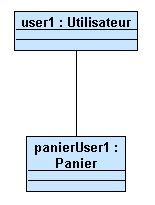
\includegraphics[scale=0.8]{diagrams/InstantaneCollectBefore.png}
	\caption{Diagramme d'objets UML  - Avant \textit{le recensement des tâches} le panier est vide}
	\end{center}
	\end{figure}
	
	\bigskip

	Ce diagramme d'objet représente un snapshot du système à un instant donné. On a ici deux instances d'Utilisateur et de Panier. En effet, le système est tout juste amorcé, l'utilisateur possède donc son panier mais il est vide.


\subsubsection {Après \textit{le recensement des tâches}}

\begin{figure}[H]
	\begin{center}
	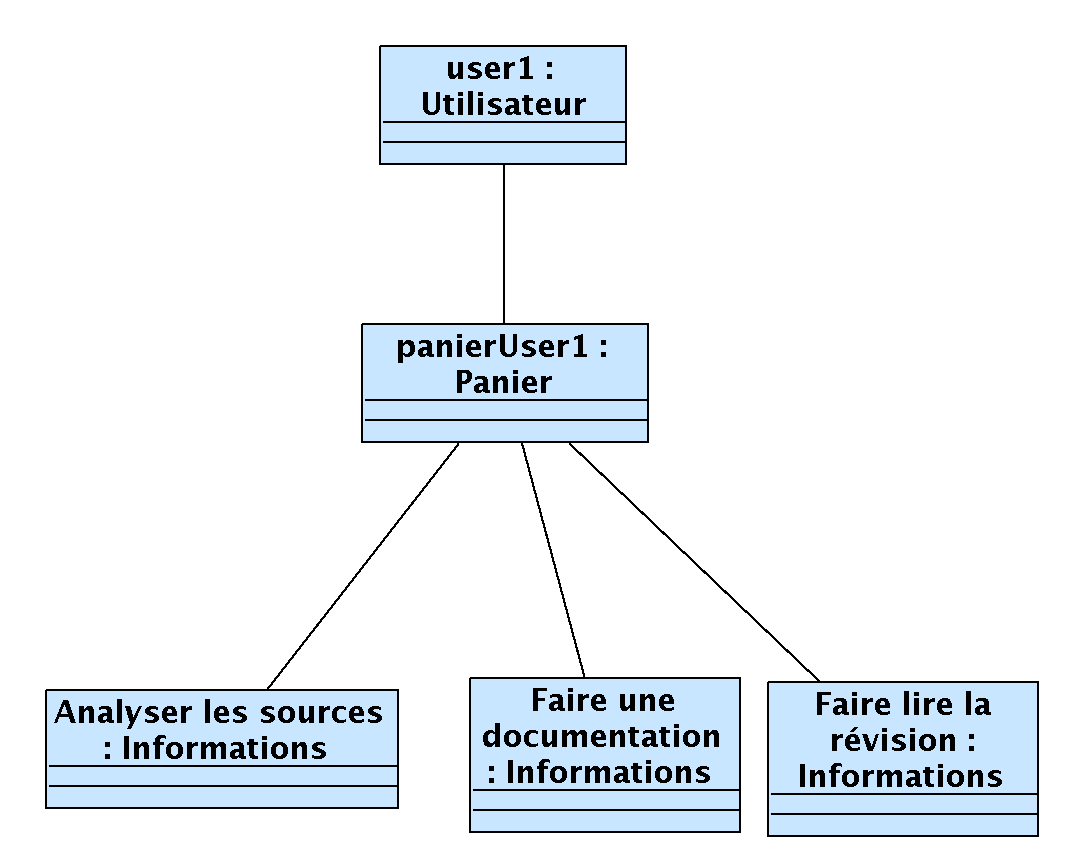
\includegraphics[scale=0.3]{diagrams/InstantaneCollectAfter.png}
	\caption{Diagramme d'objets UML  - Après \textit{le recensement des tâches}}
	\end{center}
	\end{figure}
	
	\bigskip
	

	Après \textit{Collect}, on retrouve les informations (info1, info2 et info3) que l'utilisateur a saisi après le recensement, dans le système. Celles-ci sont de la forme "information" car elles ne donneront pas forcément lieu à des tâches. Le cas d'utilisation suivant ( \textit{Process} ) explicite le traitement effectué entre "information" et "tâche".
